% !TEX TS-program = pdflatex
% !TEX encoding = UTF-8 Unicode
% {{{ setup

\documentclass[11pt,twoside]{article}

\newcommand*{\ShowAbstract}{} % Comment to hide the Abstract.
\newcommand*{\ShowFrontmatter}{} % Comment to hide the Frontmatter.
%\newcommand*{\ShowBibliography}{} % Comment to hide the Bibliography.
%\newcommand*{\ShowAppendix}{} % Comment to hide the Appendix.
%\newcommand*{\SansFontFamily}{} % Comment to use normal font.

\newcommand{\doctitle}{Path-Length Balancing in Homogeneous Operation Trees}

\usepackage[pdftex,
            pdfauthor={Dave McEwan},
            pdftitle={\doctitle},
            pdfsubject={\doctitle},
            pdfkeywords={},
            pdfproducer={},
            pdfcreator={pdflatex},
            breaklinks]{hyperref}



\usepackage[utf8]{inputenc}

\usepackage{parskip}
\usepackage{sectsty}

\usepackage[a4paper,margin=2.5cm,headheight=13.6pt]{geometry}
\usepackage{fancyhdr}
\pagestyle{fancy} % options: empty, plain, fancy
\renewcommand{\headrulewidth}{0pt}
\lhead{}\chead{}\rhead{}
\lfoot{}\cfoot{\thepage}\rfoot{}

\usepackage{url}
\usepackage{breakurl}

\usepackage{cite}

\usepackage{placeins}
\usepackage{subcaption}
\usepackage{multirow}
\usepackage[page]{appendix}

\ifdefined\SansFontFamily
    % Font for section titles.
    \allsectionsfont{\sffamily\mdseries\upshape}

    % Font for the "Appendices" title.
    \let\appendixpagenameorig\appendixpagename
    \renewcommand{\appendixpagename}{\sffamily\appendixpagenameorig}
\fi

\usepackage[usenames,svgnames]{xcolor}
\definecolor{dkgreen}{rgb}{0,0.6,0}
\definecolor{gray}{rgb}{0.5,0.5,0.5}
\definecolor{mauve}{rgb}{0.58,0,0.82}
\hypersetup{
    colorlinks,
    citecolor=black,
    filecolor=black,
    linkcolor=black,
    urlcolor=black
}

\usepackage{listings}
\lstdefinelanguage{none}{
  identifierstyle=
}
\newcommand{\lstNone}{
    \lstset{language=none,
            numbers=left,
            showstringspaces=false,
            numberstyle=\tiny\color{gray},
            numbersep=5pt,
            breaklines=false,
            basicstyle=\scriptsize\ttfamily}
}

\newcommand{\lstC}{
    \lstset{language=C,
            numbers=left,
            showstringspaces=false,
            numberstyle=\tiny\color{gray},
            keywordstyle=\color{blue},
            commentstyle=\color{dkgreen},
            stringstyle=\color{mauve},
            numbersep=5pt,
            breaklines=false,
            basicstyle=\small\ttfamily}
}

\newcommand{\lstSV}{
    \lstset{language=SystemVerilog,
            numbers=left,
            showstringspaces=false,
            numberstyle=\tiny\color{gray},
            keywordstyle=\color{blue},
            commentstyle=\color{dkgreen},
            stringstyle=\color{mauve},
            numbersep=5pt,
            breaklines=false,
            basicstyle=\small\ttfamily}
}

\lstdefinelanguage{SystemVerilog}%
  {morekeywords={% reserved keywords
      always_comb,always_ff,always_latch,%
      bit,logic,int,var,%
      always,and,assign,automatic,begin,buf,bufif0,bufif1,case,casex,%
      casez,cell,cmos,config,deassign,default,defparam,design,disable,%
      edge,else,end,endcase,endconfig,endfunction,endgenerate,%
      endmodule,endprimitive,endspecify,endtable,endtask,event,for,%
      force,forever,fork,function,generate,genvar,highz0,highz1,if,%
      ifnone,incdir,include,initial,inout,input,instance,integer,join,%
      large,liblist,library,localparam,macromodule,medium,module,nand,%
      negedge,nmos,nor,noshowcancelled,not,notif0,notif1,or,output,%
      parameter,pmos,posedge,primitive,pull0,pull1,pulldown,pullup,%
      pulsestyle_onevent,pulsestyle_ondetect,rcmos,real,realtime,reg,%
      release,repeat,rnmos,rpmos,rtran,rtranif0,rtranif1,scalared,%
      showcancelled,signed,small,specify,specparam,strong0,strong1,%
      supply0,supply1,table,task,time,tran,tranif0,tranif1,tri,tri0,%
      tri1,triand,trior,trireg,unsigned,use,vectored,wait,wand,weak0,%
      weak1,while,wire,wor,xnor,xor},%
   morekeywords=[2]{% system tasks and functions
      $clog2,$onehot,%
      $bitstoreal,$countdrivers,$display,$fclose,$fdisplay,$fmonitor,%
      $fopen,$fstrobe,$fwrite,$finish,$getpattern,$history,$incsave,%
      $input,$itor,$key,$list,$log,$monitor,$monitoroff,$monitoron,%
      $nokey},%
   morekeywords=[3]{% compiler directives
      `accelerate,`autoexpand_vectornets,`celldefine,`default_nettype,%
      `define,`else,`elsif,`endcelldefine,`endif,`endprotect,%
      `endprotected,`expand_vectornets,`ifdef,`ifndef,`include,%
      `no_accelerate,`noexpand_vectornets,`noremove_gatenames,%
      `nounconnected_drive,`protect,`protected,`remove_gatenames,%
      `remove_netnames,`resetall,`timescale,`unconnected_drive},%
   alsoletter=\`,%
   sensitive,%
   morecomment=[s]{/*}{*/},%
   morecomment=[l]//,% nonstandard
   morestring=[b]"%
  }[keywords,comments,strings]%

\usepackage{graphicx}
\graphicspath{{../img/}}
\usepackage{tikz}
\usetikzlibrary{shapes, shapes.arrows}

\usepackage{amsmath}
\usepackage{amssymb}
\usepackage{mathtools}
\newcommand{\indep}{\perp\!\!\!\perp} % Define the independent symbol
\newcommand{\nindep}{\centernot{\indep}} % Define the not-independent symbol
\newcommand{\nimplies}{\centernot{\implies}} % Define the not-implies symbol
\newcommand{\niff}{\centernot{\iff}} % Define the not-iff symbol
\newcommand{\G}{\mathcal{G}} % Graph
\newcommand{\E}{\mathcal{E}} % Edges
\newcommand{\V}{\mathcal{V}} % Nodes (vertices)
\newcommand{\reals}{\mathbb{R}}
\newcommand{\rationals}{\mathbb{Q}}
\newcommand{\integers}{\mathbb{Z}}
\newcommand{\naturals}{\mathbb{N}}
\newcommand{\complex}{\mathbb{C}}
\renewcommand{\Re}{\operatorname{Re}}
\renewcommand{\Im}{\operatorname{Im}}
\renewcommand{\vec}[1]{\mathbf{#1}} % Vector as bold, not the overhead arrow.
\newcommand{\transpose}[1]{{#1}^\mathrm{T}}

\usepackage[binary-units]{siunitx}
\let\DeclareUSUnit\DeclareSIUnit
\let\US\SI
\DeclareUSUnit\ounce{oz} % Ounce
\DeclareUSUnit\inch{in} % Inch
\DeclareUSUnit\foot{ft} % 12 inches
\DeclareUSUnit\mil{mil} % Thousands of an inch
\DeclareSIUnit\dBi{dBi} % Relative to an isotropic radiator.

\newcommand{\Hrule}{\hfil \rule{0.67\linewidth}{0.4pt} \hfil \\}

\newcommand{\TODO}[1]{[\textbf{TODO} \textsl{#1}]}

\usepackage{glossaries}
\makenoidxglossaries

\usepackage{pgfgantt} % Gantt chart.
\usepackage{pdflscape} % Put pages landscape in PDF.

\usepackage{fancyref} % \fref and Fref for nicer references.

\usepackage{enumitem} % Allow list customization.



\newglossaryentry{naiive}{
    name=na\"{\i}ve,
    description={is a French loanword (adjective, form of naïf)
        indicating having or showing a lack of experience, understanding or
        sophistication}
}

\newglossaryentry{ImageNet}{
    name={ImageNet},
    description={is an ongoing research effort to provide researchers around
        the world an easily accessible image database.}
}

\newacronym{ad}{AD}{Adaptive Design}
\newacronym{ai}{AI}{Artificial Intelligence}
\newacronym{amba}{AMBA}{Advanced Microcontroller Bus Architecture}
\newacronym{api}{API}{Application Programming Interface}
\newacronym{arm}{ARM}{Acorn RISC Machine Holdings Plc}
\newacronym{ascii}{ASCII}{American Standard Code for Information Interchange}
\newacronym{aws}{AWS}{Amazon Web Services}
\newacronym{asic}{ASIC}{Application Specific Integrated Circuit}
\newacronym{bnn}{BNN}{Binarized Neural Network}
\newacronym{bsc}{BSC}{Binary Symmetric Channel}
\newacronym{cmos}{CMOS}{Complementary Metal Oxide Semiconductor}
\newacronym{cnn}{CNN}{Convolutional Neural Network}
\newacronym{cpu}{CPU}{Central Processing Unit}
\newacronym{dft}{DFT}{Discrete Fourier Transform}
\newacronym{dftst}{DFT}{Design For Testability}
\newacronym{dma}{DMA}{Direct Memory Access}
\newacronym{dtft}{DTFT}{Discrete Time Fourier Transform}
\newacronym{ea}{EA}{Evolutionary Algorithm}
\newacronym{fec}{FEC}{Forward Error Correction}
\newacronym{ff}{FF}{Flip-Flop}
\newacronym{fft}{FFT}{Fast Fourier Transform}
\newacronym{fifo}{FIFO}{First In First Out}
\newacronym{ops}{Op/s}{Operations Per Second}
\newacronym{foss}{FOSS}{Free Open Source Software}
\newacronym{fpga}{FPGA}{Field Programmable Gate Array}
\newacronym{ga}{GA}{Genetic Algorithm}
\newacronym{hdl}{HDL}{Hardware Description Language}
\newacronym{hls}{HLS}{High Level Synthesis}
\newacronym{hmm}{HMM}{Hidden Markov Model}
\newacronym{ic}{IC}{Integrated Circuit}
\newacronym{iff}{iff}{if and only if}
\newacronym{iid}{IID}{Independent Identically Distributed}
\newacronym{ip}{IP}{Intellectual Property}
%\newacronym{ip}{IP}{Internet Protocol}
\newacronym{isa}{ISA}{Instruction Set Architecture}
%\newacronym{mac}{MAC}{Media Access Control}
\newacronym{mac}{MAC}{Multiply-Accumulate}
\newacronym{ml}{ML}{Machine Learning}
\newacronym{mm}{MM}{Minimax}
\newacronym{mmu}{MMU}{Memory Management Unit}
\newacronym{lfsr}{LFSR}{Linear Feedback Shift Register}
\newacronym{lut}{LUT}{Look Up Table Cell}
\newacronym{nn}{NN}{Neural Network}
\newacronym{ocp}{OCP}{Open Core Protocol}
\newacronym{od}{OD}{Original Design}
\newacronym{ooo}{OoO}{Out-of-Order}
\newacronym{pca}{PCA}{Principle Component Analysis}
\newacronym{ppa}{PPA}{Power, Performance, Area}
\newacronym{prng}{PRNG}{Pseudo-Random Number Generator}
\newacronym{rcg}{RCG}{Rocket Chip Generator}
\newacronym{rf}{RF}{Radio Frequency}
\newacronym{rnn}{RNN}{Recurrent Neural Network}
\newacronym{rtl}{RTL}{Register Transfer Language}
\newacronym{rv}{RISC-V}{RISC-Five}
\newacronym{sa}{SA}{Simulated Annealing}
\newacronym{sbsn}{SBSN}{Stochastic Bit-Stream Neuron}
\newacronym{sgb}{SGB}{Stochastic Gradient Boosting}
\newacronym{simd}{SIMD}{Single Instruction Multiple Data}
\newacronym{soc}{SoC}{System-on-Chip}
\newacronym{sv}{SV}{System Verilog}
\newacronym{svd}{SVD}{Singular Value Decomposition}
\newacronym{svg}{SVG}{Scalable Vector Graphics}
\newacronym{svhn}{SVHN}{Street View House Numbers}
\newacronym{svm}{SVM}{Support Vector Machine}
\newacronym{tl}{TileLink}{TileLink On-Chip Interconnect}
\newacronym{ua}{uarch}{Micro Architecture}
\newacronym{us}{UltraSoC}{UltraSoC Technologies Ltd}
\newacronym{v95}{V95}{Verilog (1995)}
\newacronym{vliw}{vliw}{Very Long Instruction Word}
\newacronym{vlsi}{VLSI}{Very Large Scale Integration}


\graphicspath{{./img/}}
\renewcommand{\fancyrefdefaultformat}{plain}

\author{Dave McEwan}

\title{WIP: \doctitle}

\date{}

% }}} setup

\begin{document}
\ifdefined\SansFontFamily
    % Font for main text.
    \sffamily
\fi

\ifdefined\ShowFrontmatter
    \maketitle

    \ifdefined\ShowAbstract
        \begin{abstract}
This paper explores the problem of path-length balancing in k-ary trees.
A simple technique is presented to reduce the differences in the path-lengths
between inputs which is named ``port-mapping''.
Several variants of port-mapping are given and compared.
This is directly related to several problems in \gls{asic} design including OR
tree implementation, counting the number of set bits in a vector, and finding
the sum or product of a list of results.

%Firstly the central ideas and notation are introduced with examples.
%Secondly a handful of port-mapping algorithms are explained.
%Thirdly some results are presented.
        \end{abstract}
    \fi
\fi

\setcounter{tocdepth}{2}
%\tableofcontents

\section{Introduction}
The problem of balancing the lengths of operation trees is of interest to
several fields, in particular \gls{asic} layout design where a longer path
between the output of one \gls{ff} to the input of another \gls{ff} means that
the clock must be run more slowly in order to avoid metastability and unknown
data issues.
In this paper the length of a path refers primarily to the number of logic cells
passed through (e.g. 5 AND cells), rather than the physical length of the path
(e.g. \SI{0.5}{\mm}).
The operation tree input vector $\vec{x}$ is composed of $w$ elements.
The values applied to the input vector also form a vector $\vec{x}$.
The output scalar $f(\vec{x})$ of the operation tree is a function of the values
applied to the input elements.
Each operation must take the same number of inputs $b$, which in \gls{asic}
layout corresponds to all operations being implemented with the same cell,
e.g. for a tree of two input OR cells $b = 2$.
It is assumed to be legal to tie any number of inputs to a constant value,
and that when less than two inputs to the operation are constant then the
operation may be removed completely.

A homogenous series of operations may be arranged as a tree if the operation is
both commutative and associative.
Common examples include AND, OR, XOR, ADD, and MULTIPLY.
%Common operations which may not be arranged as such include NAND, NOR, NXOR,
%SUBTRACT, and DIVIDE.
%Without loss of generallity we may use an OR tree for all demonstrations of the
%port-mapping technique where the output is defined by
%$f(\vec{x}) = x_0 \lor x_1 \lor \ldots \lor x_{w-1}$.
%In the Verilog language this may be written as \texttt{wire f = |x;}.
Two implementations of the 4-input OR function are shown in \fref{fig:OR_b2_w4}
to demonstrate the terms path-length and balancing.
All OR operations use $b=2$ inputs, and each implementation uses $3$
operations.

In \fref{fig:OR_b2_w4_maxbal} all $4$ inputs `cross' an identical
number of $2$ operations to reach the output, known as the path length.
In contrast in \fref{fig:OR_b2_w4_unbal} $x_3$ only crosses one
operation whereas $x_0$ and $x_1$ cross three operations.
In an \gls{asic} layout this would mean that all inputs in
\fref{fig:OR_b2_w4_maxbal} may propagate their voltage faster toward the net
$f$ than inputs $x_0$ and $x_1$ in \fref{fig:OR_b2_w4_unbal}, which means that
the balanced design will be able to run at a faster clock speed.
This suggests that a balanced implementation may be a better choice for a fast,
high performance design whereby the speed is limited by the maximum path length.
Alternatively, to make both designs function at the same clock speed some
additional buffering and amplifiying components may be added to the unbalanced
design, at the expense of the additional area and power consumed, in order to
compensate for the parasitic elements associated with the higher gate delays on
in inputs $0$ and $1$.
This suggests that a balanced implementation may be a better choice for a
physically smaller and lower power design.

\begin{figure}[h]
    \begin{subfigure}[t]{0.5\textwidth}
        \centering
        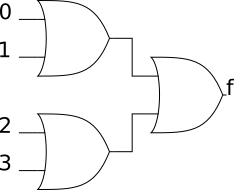
\includegraphics[width=0.5\textwidth]{OR_b2_w4_maxbal.png}
        \caption{Maximally balanced.
                 \label{fig:OR_b2_w4_maxbal}}
    \end{subfigure}%
    ~
    \begin{subfigure}[t]{0.5\textwidth}
        \centering
        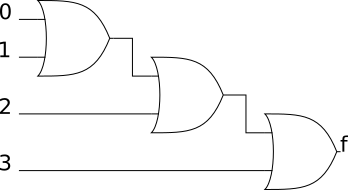
\includegraphics[width=0.75\textwidth]{OR_b2_w4_unbal.png}
        \caption{Maximally unbalanced.
                 \label{fig:OR_b2_w4_unbal}}
    \end{subfigure}

    \caption{OR trees with $b=2$ and $w=4$. \label{fig:OR_b2_w4}}
\end{figure}

This problem may be formulated as a rooted k-ary tree graph where the output $f$
is the root node, and the input vector $\vec{x}$ is the leaf nodes.
Let a vector $\vec{d}$ be formed by the distances from the leaf nodes to the
root node.
E.g. In \fref{fig:OR_b2_w4_maxbal} it can be seen that
$\vec{d} = \transpose{(2\ 2\ 2\ 2)}$ and in \fref{fig:OR_b2_w4_unbal} it can
be seen that $\vec{d} = \transpose{(3\ 3\ 2\ 1)}$.

\begin{align} \label{eq:d}
\vec{d}_i = d(\vec{x}_i, f)
\end{align}

It can be supposed that a faster circuit implementation is achieved by
minimizing $\max(\vec{d})$, and that a lower power \gls{asic} implementation
is achieved by minimizing the total path length $t = \sum \vec{d}$.

By using a tree of logic like \fref{fig:OR_b2_w4_maxbal} rather than a chain of
operations like \fref{fig:OR_b2_w4_unbal}, it can be seen that
$\max(\vec{d}) = log_b\lceil \log_bw \rceil$.
A chain of operations like \fref{fig:OR_b2_w4_unbal} which is a maximally
unbalanced tree may be used to give an upper bound $t \leq t_{\text{max}}$.
A maximally balanced tree may be used to find an approximation of the lower
bound $t \geq w\log_bw$.
An exact integer solution $t_{\text{min}}$ may be found for the lower bound by
observing that each leaf node will have a path length equal to either
$\lfloor \log_bw \rfloor$ or $\lceil \log_bw \rceil$.

To reduce the about of notation let $n = b^{\lceil \log_bw \rceil}$, i.e. the
next closest power of $b$ which is greater than or equal to $w$, and let
$p = b^{\lfloor \log_bw \rfloor}$, i.e. the previous closest power of $b$
which is less than or equal to $w$.
It can then be calculated that the number of leaf nodes with a path length
equal to $\lfloor \log_bw \rfloor$ is given by
$\#_{\text{floor}}=p-\lceil \frac{w-p}{b-1} \rceil$.

\begin{align}
\label{eq:t_lower}
t \geq t_{\text{min}} &= \
(\#_{\text{floor}})\lfloor \log_bw \rfloor + \
(w-\#_{\text{floor}})\lceil \log_bw \rceil \\
\label{eq:t_upper}
t \leq t_{\text{max}} &= \frac{w(w+1)}{2}-1
\end{align}
% Interestingly, it can be shown that for trees with $b=2$ the port numbers can
% be represented in Gray code and the results for the usual `forward' case are
% identical to BASE2FWD, and the results for the digit reversed case are
% identical to BASE2REV.

\begin{figure}[h]
    \centering
    \begin{subfigure}[t]{0.9\textwidth}
        \centering
        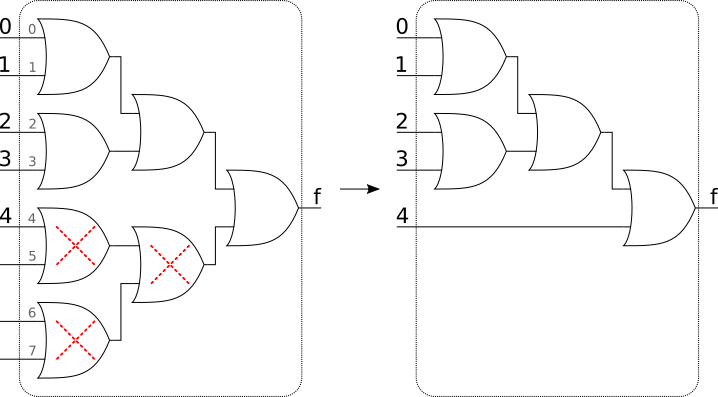
\includegraphics[width=0.67\textwidth]{OR_b2_w5_FWD.png}
        \caption{OR tree with FWD port mapping.
                 $\vec{d} = \transpose{(3\ 3\ 3\ 3\ 1)}$,
                 $t = 13$.
                 \label{fig:OR_b2_w5_FWD}}
    \end{subfigure}

    \begin{subfigure}[t]{0.9\textwidth}
        \centering
        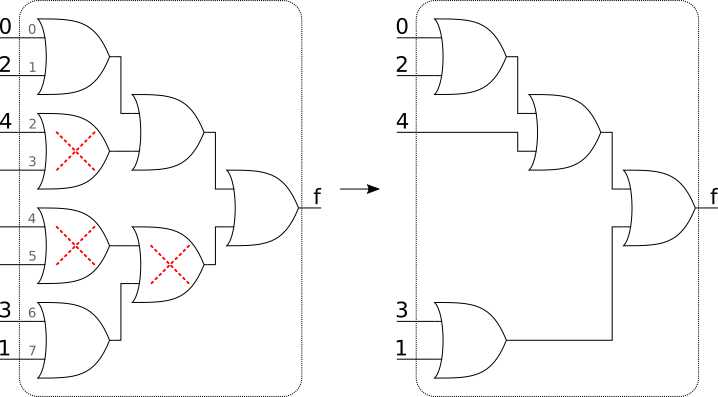
\includegraphics[width=0.67\textwidth]{OR_b2_w5_PINGPONG.png}
        \caption{OR tree with PINGPONG port mapping.
                 $\vec{d} = \transpose{(3\ 2\ 3\ 2\ 2)}$,
                 $t = 12$.
                 \label{fig:OR_b2_w5_PINGPONG}}
    \end{subfigure}

    \begin{subfigure}[t]{0.9\textwidth}
        \centering
        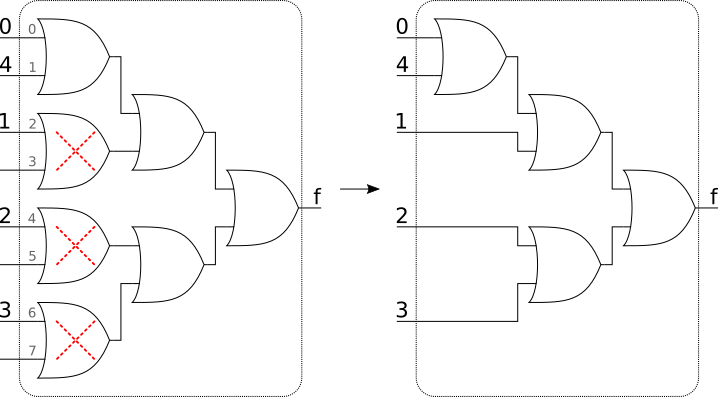
\includegraphics[width=0.67\textwidth]{OR_b2_w5_BSTRIDE.png}
        \caption{OR tree with BSTRIDE port mapping.
                 $\vec{d} = \transpose{(3\ 2\ 2\ 2\ 3)}$,
                 $t = 12$.
                 \label{fig:OR_b2_w5_BSTRIDE}}
    \end{subfigure}

    \begin{subfigure}[t]{0.9\textwidth}
        \centering
        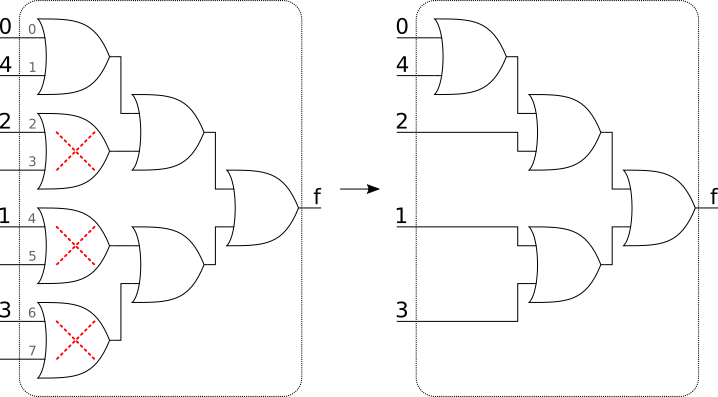
\includegraphics[width=0.67\textwidth]{OR_b2_w5_BASEBREV.png}
        \caption{OR tree with BASEBREV port mapping.
                 $\vec{d} = \transpose{(3\ 2\ 2\ 2\ 3)}$,
                 $t = 12$.
                 \label{fig:OR_b2_w5_BASEBREV}}
    \end{subfigure}

    \caption{OR trees with $b=2$ and $w=5$. \label{fig:OR_b2_w5}}
\end{figure}

\Fref{fig:OR_b2_w5} demonstrates that for the example of $w=5,\ b=2$ the
total path length can be changed simply by changing the order in which inputs
are allocated to the operation tree.
The indexes of the leaf nodes are shown in gray smaller text and are numbered
in the natural order.
The function input indices are shown in black larger text and are numbered
according to the named algorithms.
Leaf nodes which are not used are unlabelled to signify that they are tied to a
constant equal to the identity element and that any operations depending on
them may be removed.
This means that in \gls{asic} development the optmization may be performed at
the \gls{rtl} (e.g. Verilog) level.
OR gates which may be removed are marked with a large red cross.
The right hand diagrams show the resulting implementations for this example, all
of which use four operations and have a $\max(\vec{d}) = 3$.

\clearpage
\section{Port-Mapping Algorithms}

Each of these algorithms $a$ performs a bijective mapping from a leaf node
index $x$ onto a function input index $y$,
i.e. $x,y \in \integers_0,\ a: x \to y,\ a^{-1}: y \to x$.
%The inverse function $a^{-1}$ maps a function input index to a leaf node index.
Leaf nodes which do not have a corresponding function index,
i.e. $a^{-1}(y) \geq w$, are tied to a constant of the identity element which
allows operations to be removed.
An operation may be removed if less than two of its inputs are constant.

For trees where $b>2$ it is possible for an individual operation to have more
than one non-constant input, and one or more constant inputs meaning
it is only partially used and ideally would be relaced with a smaller cell.
For this reason the concept of using a non-linear weighting $\alpha$ for each
operation is introduced, i.e. the distance across two adjacent nodes
$d(a, b) = ( \frac{\text{\# connected inputs}}{b} )^\alpha$.
Each result is therefore fully specificed by $t_{w,\alpha,b,a}$.
Note that the bounds given by \fref{eq:t_lower} and \fref{eq:t_upper} only hold
for $b=2$ or $\alpha=0$.

\begin{figure}[h]
    \begin{subfigure}[b]{0.5\textwidth}
        \centering
        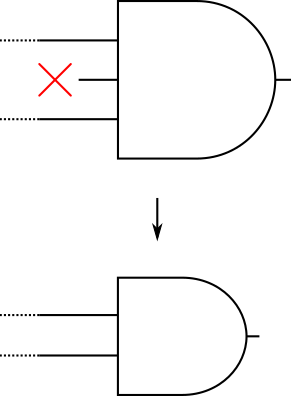
\includegraphics[width=0.5\textwidth]{alpha_demo.png}
        \caption{3AND with only 2 used inputs may be converted to a 2AND.
                 \label{fig:alpha_demo}}
    \end{subfigure}%
    ~
    \begin{subfigure}[b]{0.5\textwidth}
        \centering
        \begin{tabular}{ l | c }
            $\alpha$    & $d(\vec{x}_i, 2AND),\quad b=3$   \\
            \hline
            $-2$        & $2.25$        \\
            $-1$        & $1.5$         \\
            $-0.5$      & $1.225$       \\
            $0$         & $1$           \\
            $0.5$       & $0.816$       \\
            $1$         & $\frac{2}{3}$ \\
            $\varphi$   & $0.519$       \\
            $2$         & $0.444$       \\
%            $e$         & $0.332$       \\
%            $\pi$       & $0.280$       \\
        \end{tabular}
        \caption{Example distances across a single operation for different
            values of $\alpha$.
            \label{tab:alpha_values}}
    \end{subfigure}
\end{figure}

In typical models where cells with less inputs are smaller faster, and incur
less capacitance, $\alpha$ is set to greater than $1$.
For example it may be the case that a 2AND cell incurs less than $\frac{2}{3}$
of the capacitance per input of a 3AND cell.
The golden ratio defined as $\varphi = \frac{1 + \sqrt 5}{2}$ is though to be a
reasonable initial approximation.
For \gls{asic} layout comparisons the chosen value of $\alpha$ is dependent on
the process node and cell library which will be used for implementation.

The \textit{FWD} algorithm is the simplest port-mapping algorithm and perhaps
the na\"{\i}ve method.
\begin{align} \label{eq:a_fwd}
a_{\textsc{fwd}}(i) = a_{\textsc{fwd}}^{-1}(i) = i
\end{align}
For a more intuitive comparison of values it is useful to scale $t$ by the
number of inputs and the result of the \textit{FWD} algorithm to give a measure
of the reduction in total capacitance given by use of an algorithm other than
the na\"{\i}ve method, i.e,
\begin{align} \label{eq:u}
u_{w,\alpha,b,a} = w - \frac{wt_{w,\alpha,b,a}}{t_{w,\alpha,b,\textsc{fwd}}}
\end{align}
For a lower total capacitance we want $u$ to be as high as possible.

The \textit{BASEBREV} algorithm takes a function input index represented in
base $b$ and zero-extended to $m = \log_bn$ digits, and reverses the order of
the digits.
\begin{align}
\text{let}\quad i &= \sum\limits_{k = 0}^{m-1} x_k b^k \\
\label{eq:a_basebrev}
a_{\textsc{basebrev}}(i) = a_{\textsc{basebrev}}^{-1}(i) &= \
    \sum\limits_{k = 0}^{m-1} x_{m-k-1} b^k
\end{align}

The \textit{PINGPONG} algorithm allocates function input indices to
alternating ends of the ordered set of leaf node indices.
The \textit{PONGPING} algorithm is simply the reverse of the  \textit{PINGPONG}
process.
\begin{align}
\label{eq:a_pingpong}
a_{\textsc{pongping}}^{-1}(i) = a_{\textsc{pingpong}}(i) &= \
    2i\ \text{if}\ (i < \frac{n}{2})\ \text{else}\ 2(n-i)-1 \\
\label{eq:a_pongping}
a_{\textsc{pingpong}}^{-1}(i) = a_{\textsc{pongping}}(i) &= \
    n-\frac{i+1}{2}\ \text{if}\ (i \bmod 2)\ \text{else}\ \frac{i}{2}
\end{align}

The \textit{STRIDEB} algorithm allocates function input indices in strides of
$b$, restarting at the lowest index when it walks off the upper end.
The \textit{STRODEB} algorithm is simply the inverse of the \textit{STRIDEB}
process.
\begin{align}
\label{eq:a_stride}
a_{\textsc{strodeb}}^{-1}(i) = a_{\textsc{strideb}}(i) &= \
    (ib \bmod n) + \left\lfloor \frac{ib}{n} \right\rfloor \\
\label{eq:a_strode}
a_{\textsc{strideb}}^{-1}(i) = a_{\textsc{strodeb}}(i) &= \
    \Big( \left\lfloor \frac{in}{b} \right\rfloor \bmod n \Big) + \
    \left\lfloor \frac{i}{b} \right\rfloor
\end{align}

The \textit{GRAYFWD} and \textit{GRAYREV} algorithms use n-ary generalized
(n,k)-Gray codes to allocate indices. i.e. using
$(b, \lceil\log_bw\rceil)$-Gray codes.
\begin{align}
\text{let}\quad i &= \sum\limits_{k = 0}^{m-1} x_k b^k \\
\text{let}\quad j &= \left\lfloor \frac{i}{b^k} \right\rfloor \\
\label{eq:a_grayfwd}
a_{\textsc{grayfwdi}}^{-1}(i) = a_{\textsc{grayfwd}}(i) &= \
    \sum\limits_{k = 0}^{m-1} y_k b^k \\
\label{eq:a_grayrev}
a_{\textsc{grayrevi}}^{-1}(i) = a_{\textsc{grayrev}}(i) &=  \
    \sum\limits_{k = 0}^{m-1} y_{m-k-1} b^k \\
y_k &= \Big( j - \left\lfloor \frac{j}{b} \right\rfloor \Big) \bmod b
\end{align}
The \textit{GRAYREV} algorithm reverses the order of the base $b$ digits as
compared to the values returned by \textit{GRAYFWD}.
The inverse functions have not been implemented or tested here.

These are just a few named examples of the $n!$ possible algorithms as it is
not feasible to test all possibile algorithms.
The number of possible non-equivalent algorithms may be reduced to
$\frac{n!}{\frac{n}{b} \times (\frac{n}{b})!}$ by observing that
rearranging the inputs to a single operation at the top of the operation tree
always gives equivalent results, however, this is still an infeasibly large
number of algorithms to test exhaustively.

\clearpage
\section{Results}
% Generate figures with:
%   ./treebalance.py -p --wmax 300
%   OR
%   make plots
\begin{figure}[h]
    \centering
    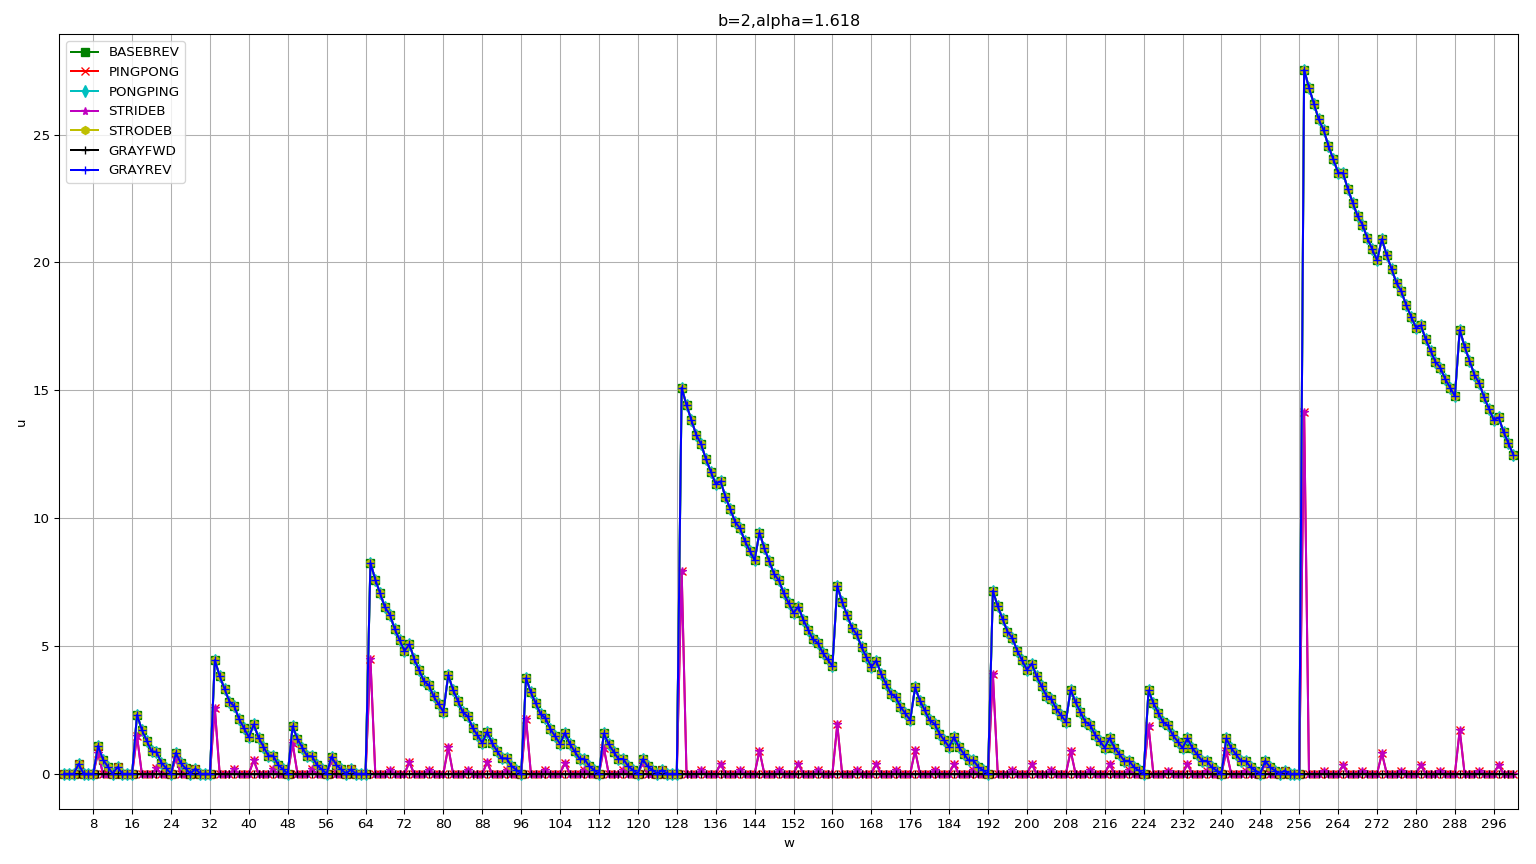
\includegraphics[width=0.93\textwidth]{b=2,alpha=1_618.png}
    \caption{Total path length savings compared to $a_{\textsc{fwd}}$
             where only 2-input cells are available.
             \label{fig:b=2,alpha=1_618}}
\end{figure}
\vfill
\begin{figure}[h]
    \centering
    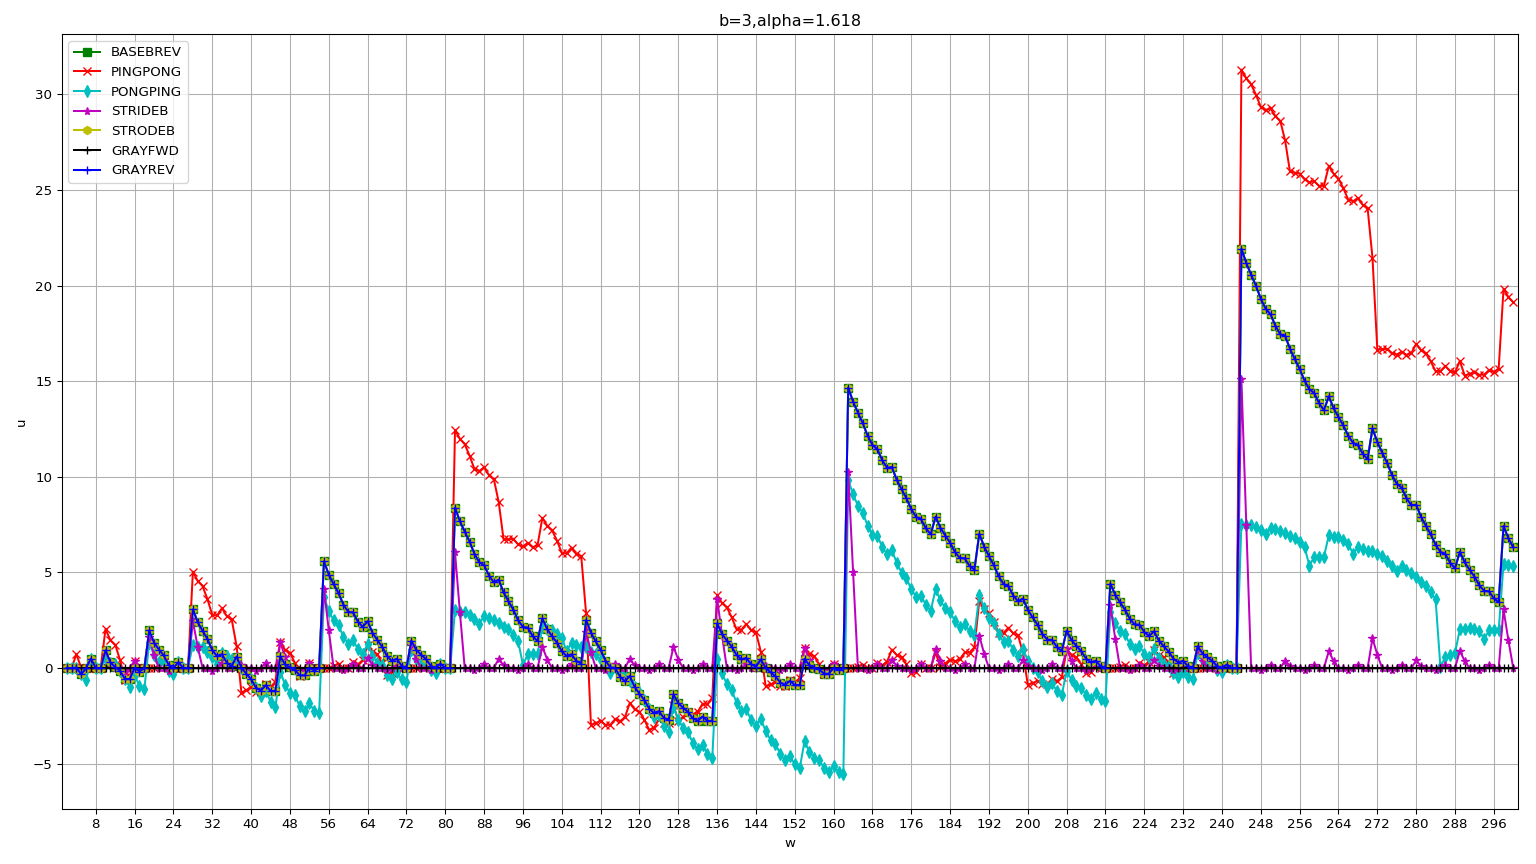
\includegraphics[width=0.93\textwidth]{b=3,alpha=1_618.png}
    \caption{Total path length savings of compared to $a_{\textsc{fwd}}$ where
             3-input cells are available.
             \label{fig:b=3,alpha=1_618}}
\end{figure}

\begin{figure}[h]
    \centering
    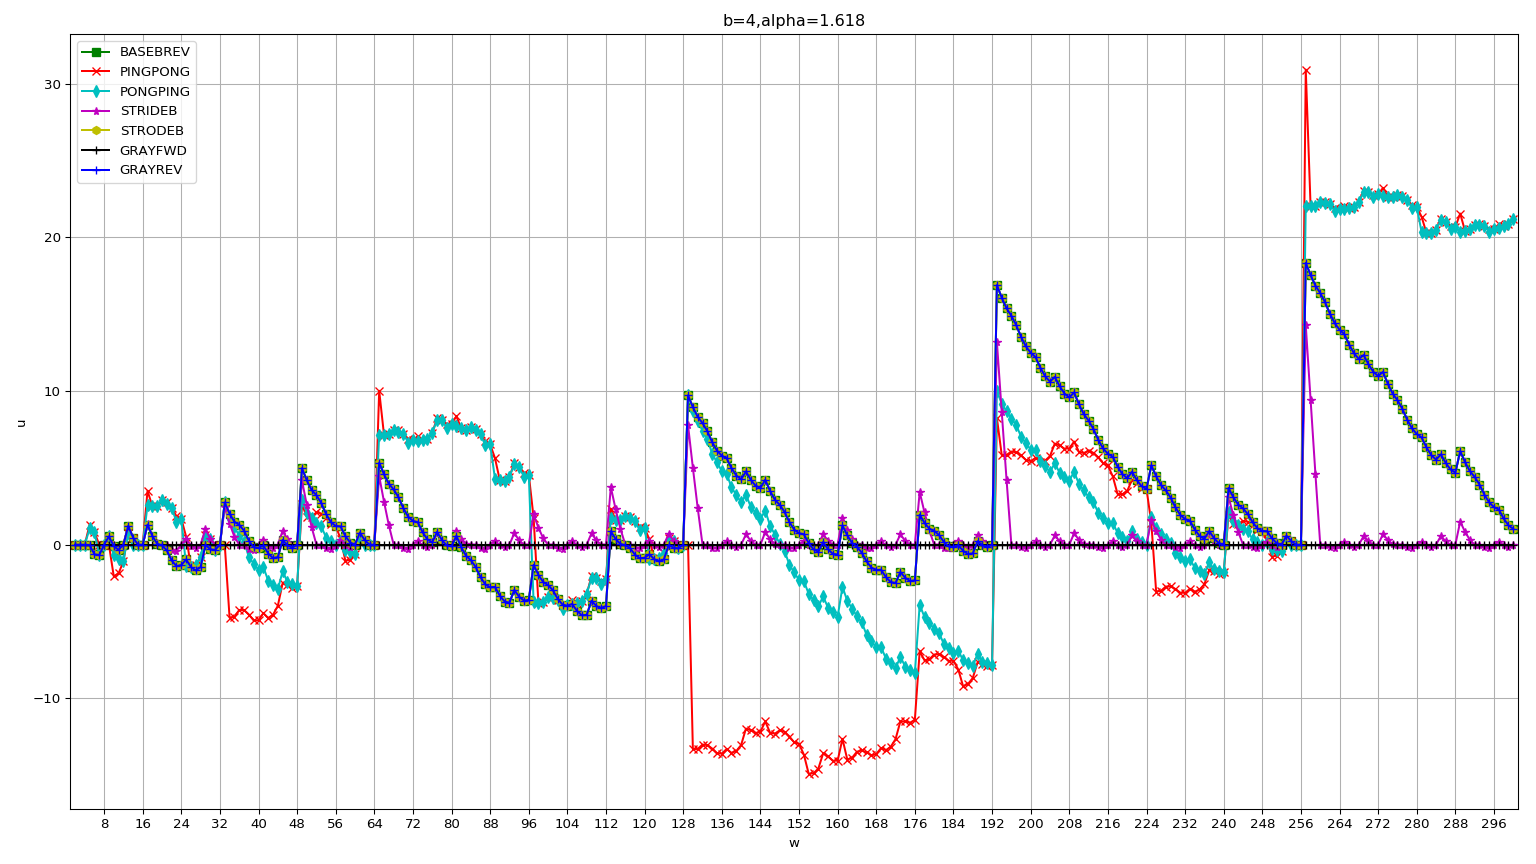
\includegraphics[width=0.93\textwidth]{b=4,alpha=1_618.png}
    \caption{Total path length savings of compared to $a_{\textsc{fwd}}$ where
             4-input cells are available.
             \label{fig:b=4,alpha=1_618}}
\end{figure}
\vfill
\begin{figure}[h]
    \centering
    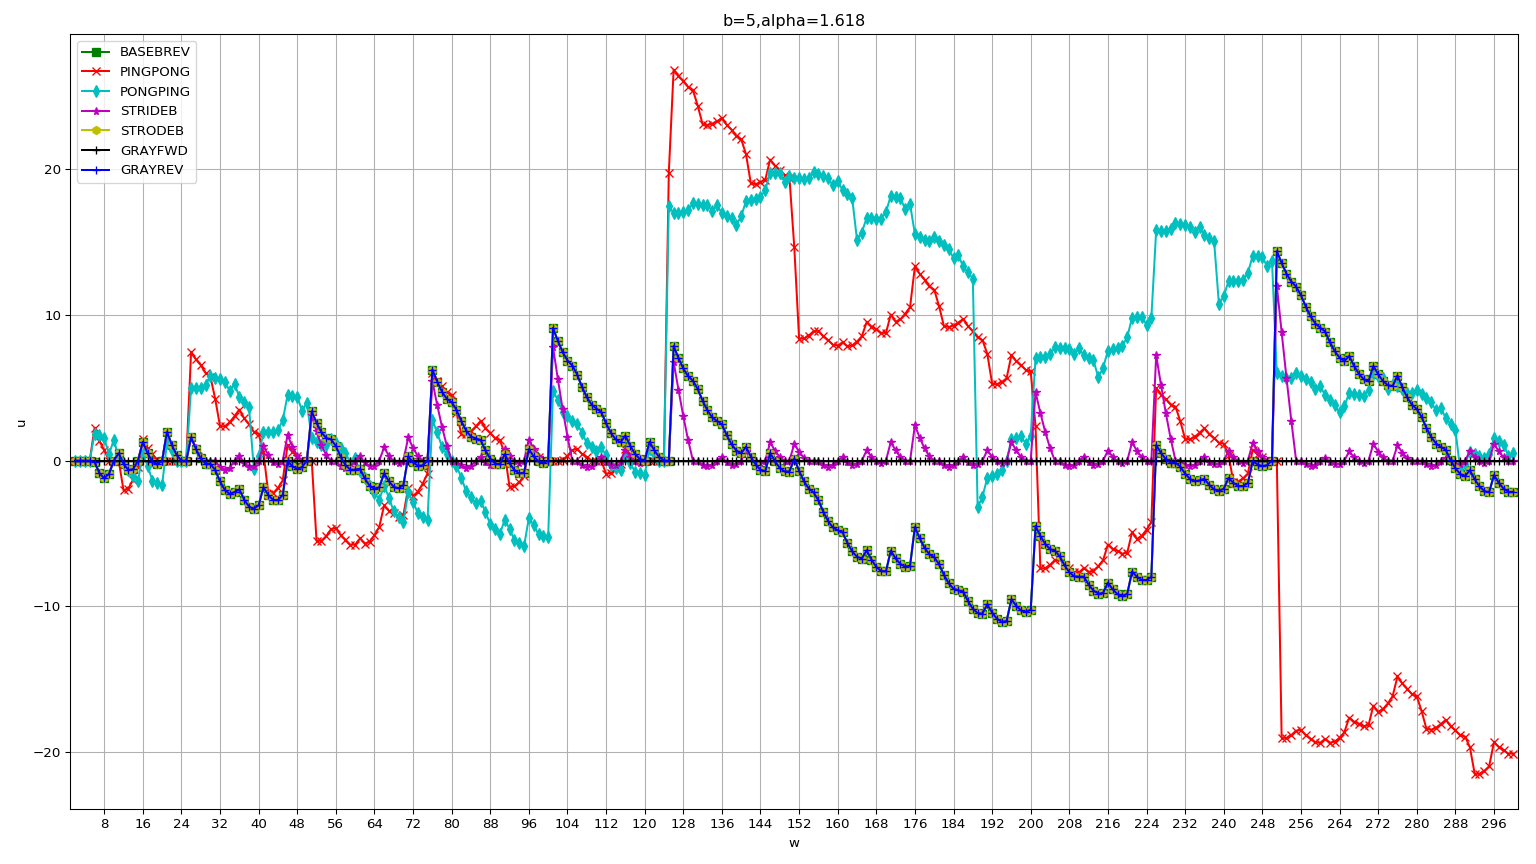
\includegraphics[width=0.93\textwidth]{b=5,alpha=1_618.png}
    \caption{Total path length savings of compared to $a_{\textsc{fwd}}$ where
             5-input cells are available.
             \label{fig:b=5,alpha=1_618}}
\end{figure}
\clearpage
These figures show that for operation trees where the number of leaf nodes is
not an integer power of $b$ it is possible to reduce the total path length, and
the associated capacitance simply by changing the order in which function
indices are assigned to leaf node indices.
The biggest potential savings appear where $w$ is a power of $b$ plus 1.

\TODO{Discuss comparative advantages}
\TODO{Non-trivial estimation of optimal choice}

For the special case $b=2$ where $\alpha$ has no effect and the bounds of $t$
are known it makes sense to compare against the lower bound rather than the
result of $a_{\textsc{fwd}}$
i.e. $v_{w,a} = w - \frac{w-wt_{w,a}}{t_{\text{min}}}$,
as shown in \fref{fig:b=2}.
Here it can be seen that $a_{\textsc{fwd}}$ has the highest total path length
and $a_{\textsc{basebrev}}$ is among a collection of algorithms which is always
optimal.
\begin{figure}[h]
    \centering
    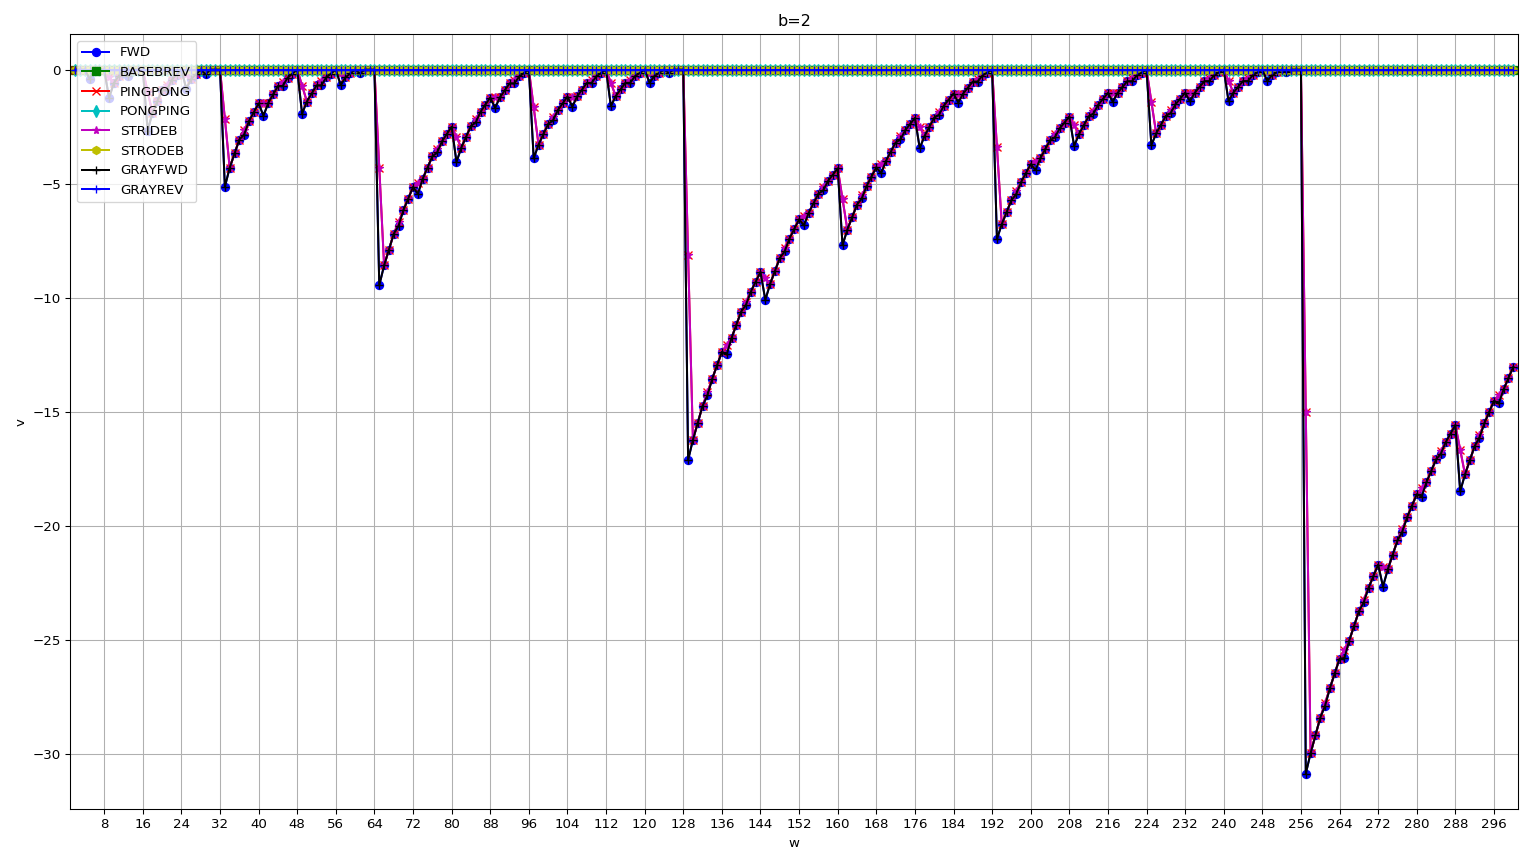
\includegraphics[width=1.0\textwidth]{b=2.png}
    \caption{Total path length savings compared to optimal algorithm where only
             2-input cells are available.
             Higher is better, $v=0$ is optimal.
             \label{fig:b=2}}
\end{figure}

The case where only 2-input cells are available is not uncommon for more complex
operations such as multipliers.
For simpler operations such as OR many cell libraries will have cells with more
than 2 inputs available, in which case an appropriate value of $\alpha$ must be
chosen in order to perform a meaningful comparison.

%\TODO{ref TSMC, GF cell lib specs}
%\TODO{ref Xilinx, Altera, Lattice primitive cell specs}
\TODO{practical demonstration with FPGA?}

\TODO{Zero cost in synthesis computation time.}
\TODO{Zero cost in silicon area.}
\TODO{Zero cost in max path length.}
\TODO{RTL/HDL level.}

%\clearpage
%\section{Conclusions}

% {{{ epilog

\ifdefined\ShowBibliography
\clearpage
\bibliographystyle{plain}
\addcontentsline{toc}{section}{Bibliography}
\bibliography{../refs}{} % refs.bib
\fi

\ifdefined\ShowAppendix \clearpage \begin{appendices} % {{{
    \addappheadtotoc
    %\appendixpage


%\section{Lists}
%
%\listoffigures
%
%\listoftables

\end{appendices} \fi % }}}

% }}} epilog

\end{document}
